\documentclass{beamer}
 
\usepackage[utf8]{inputenc}
 
 
\title{Propagation of Voltage in a Neuron}
\subtitle{The Cable Equation}
\author{Darice Guittet, Elise Niedringhaus, Sarah Liddle}
\date{Fall 2017}
 
 
 
\begin{document}
 
\frame{\titlepage}
 
\begin{frame}
\frametitle{Overview}
1. Motivation \newline \newline
2. Neuronal Cable Equation \newline \newline
3. Passive Membrane (Linear Cable Equation) \newline \newline
4. Bi-stable Ion Channels
\end{frame}

\begin{frame}
\frametitle{How Do Neurons Communicate?}
\begin{columns}
    \begin{column}{.5\textwidth}
    Within one cell
    \begin{itemize}
	\item Electrochemical signals
	\item Membrane Potential: $\Delta V_m = V_i - V_e$
	\item Ions: charge-carriers
	\item Ion Channels in Membrane \newline
	\end{itemize}
	Between cells
	\begin{itemize}
	\item Neurotransmitters
\end{itemize}
    \end{column}
    
    \begin{column}{.5\textwidth}
    \begin{figure}[H]\label{neuron}
    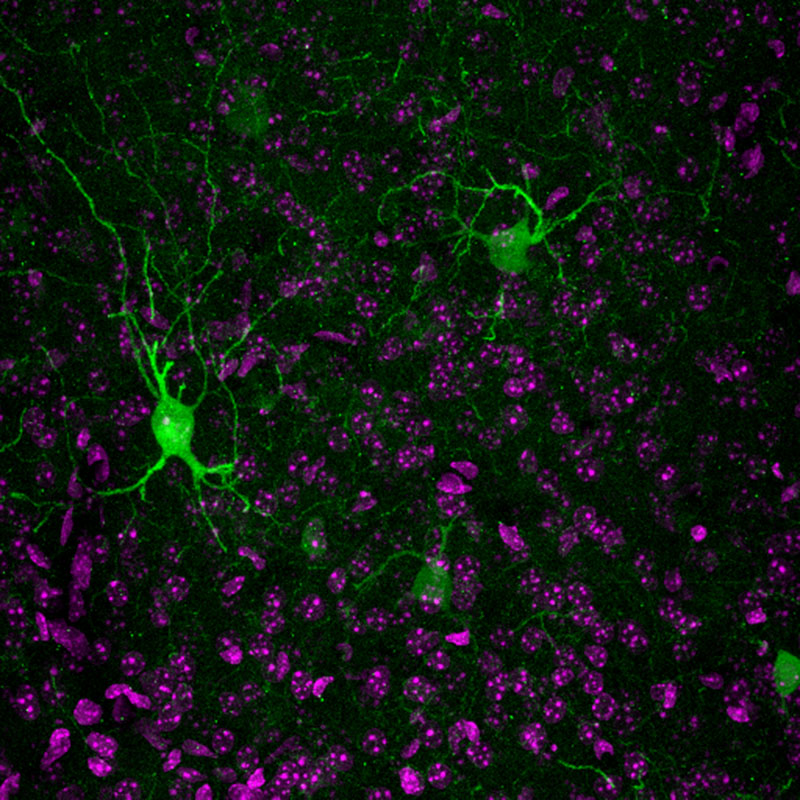
\includegraphics[width=\textwidth]{OConnor-InhibitoryInterneurons1}
	\caption{Mouse neurons, 40X. Bosch Institute Advanced Microscopy Facility, The University of Sydney}
    \end{figure}
    
    \end{column}
  \end{columns}
\end{frame}

\begin{frame}
\frametitle{Action Potentials}
\begin{figure}
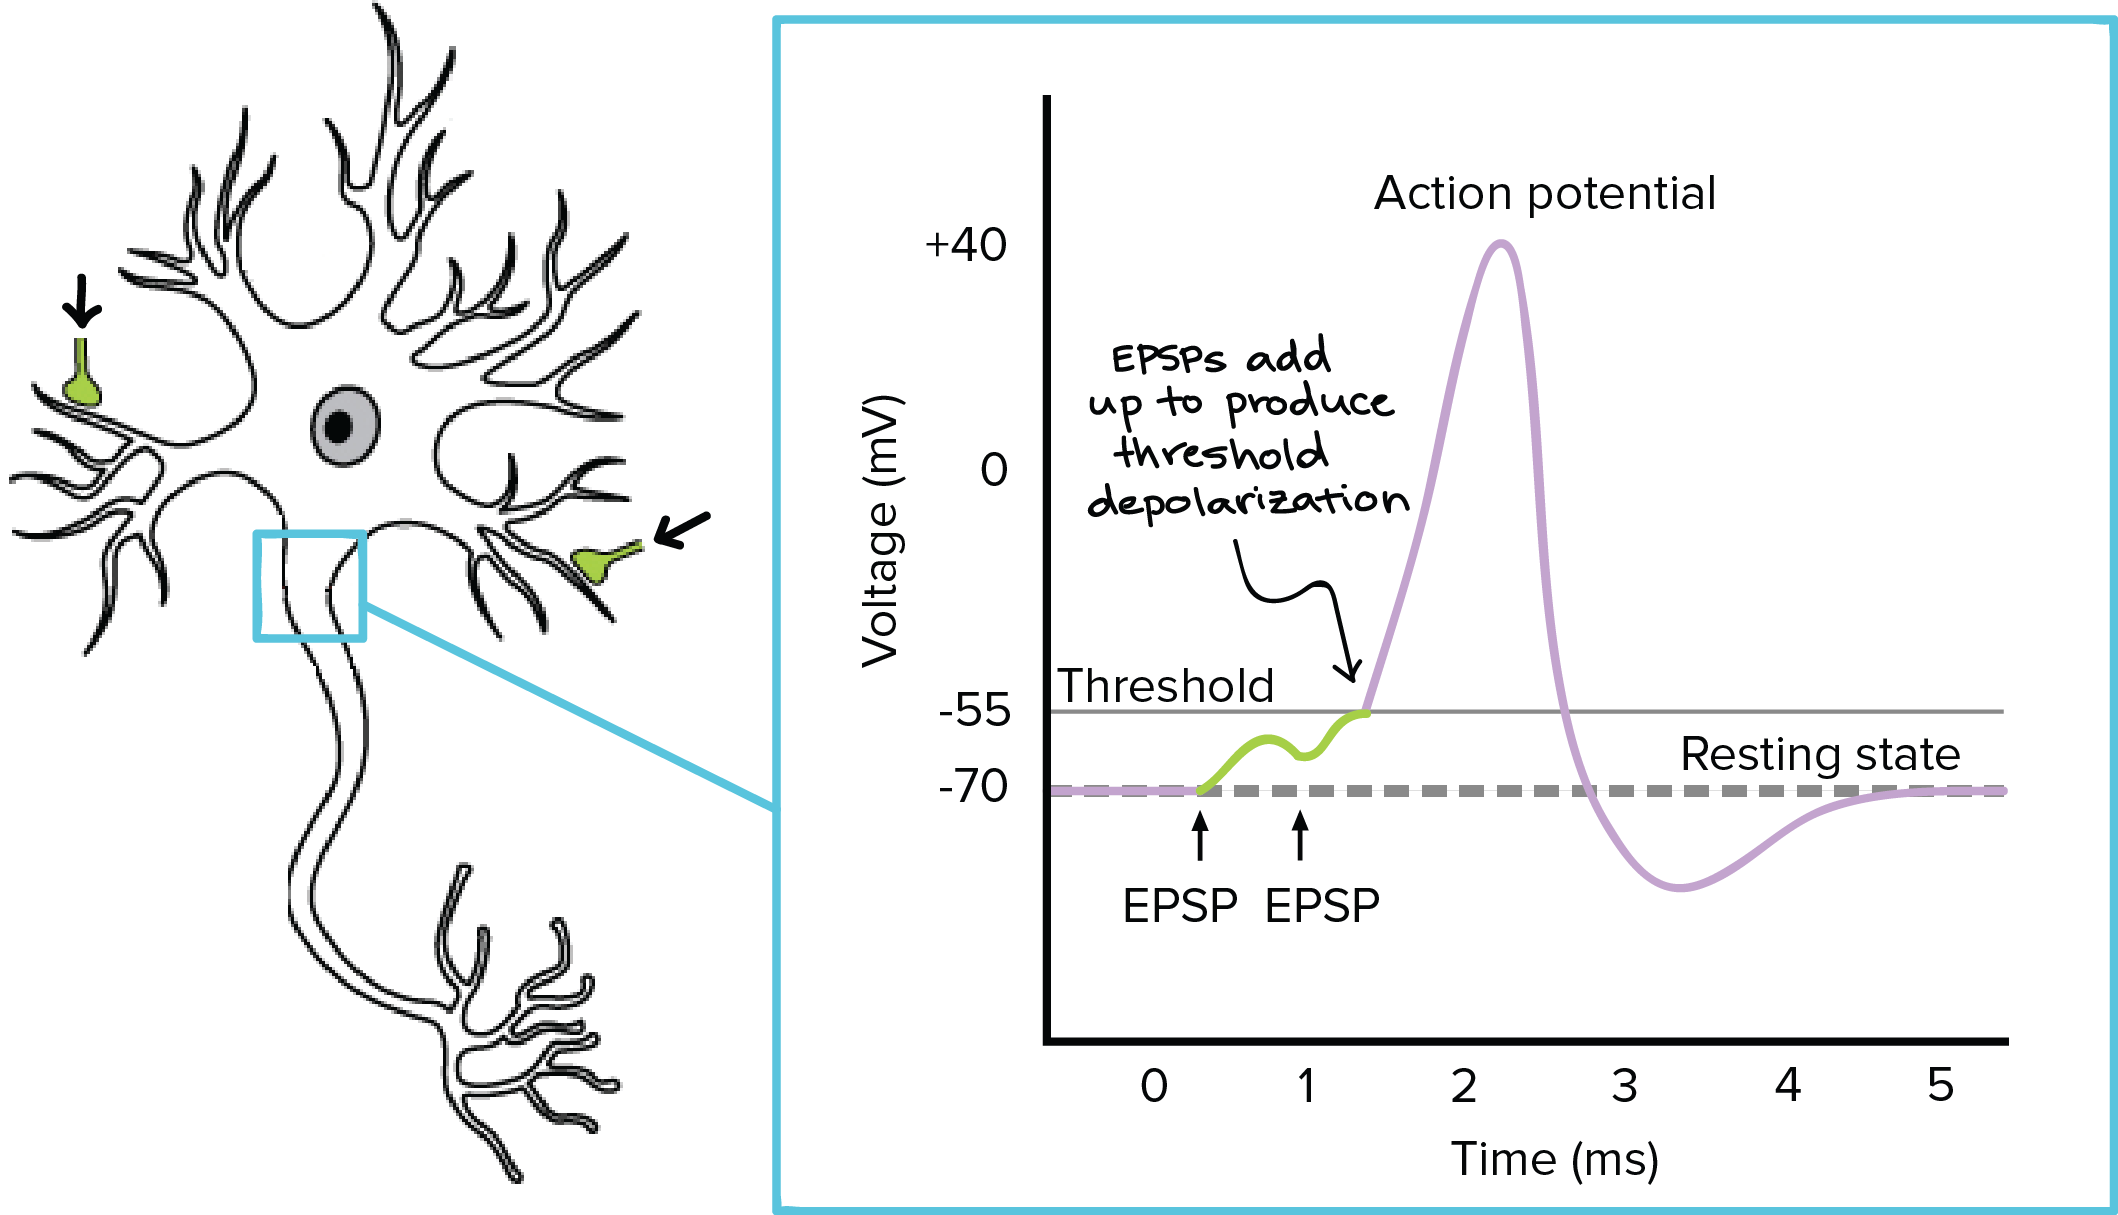
\includegraphics[width=\textwidth]{actionpotential}
\caption{Changes in axonal membrane voltage due to an action potential. Image from Khan Academy}
\end{figure}
\end{frame}

\begin{frame}
\frametitle{Hodgkin-Huxley's Neuronal Cable Model}
\begin{columns}
\begin{column}{.65\textwidth}
\begin{figure}
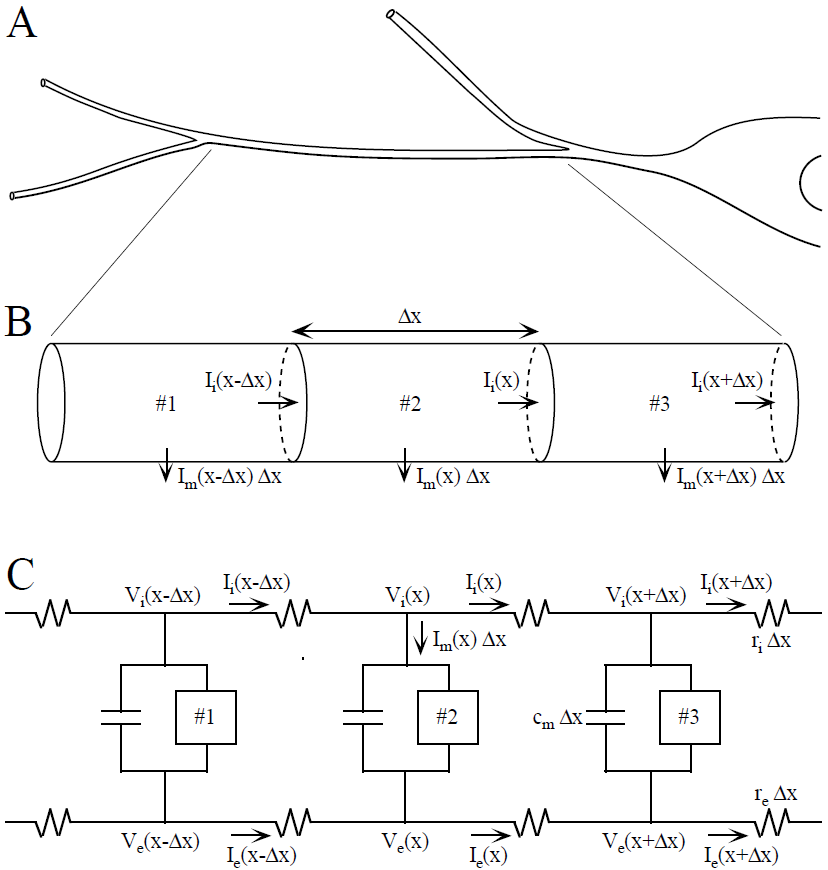
\includegraphics[scale=0.35]{NeuronalCableModel}
\caption{Differential membrane patches as circuit. Image from jh.edu/motn}
\end{figure}
\end{column}

\begin{column}{.45\textwidth}
\begin{itemize}
	\item{1-D \& Ohmic assumption}
	\item{Intracellular current}
	\item{Extracellular current}
	\item{Membrane current}
	\item{Membrane as capacitor}
	\item{Ion channels as conductances}
	\item{Length Constant: $\lambda = \sqrt{\frac{r_m}{r_i+r_e}}$}
	\item{Time Constant: $r_mC_m$ }
\end{itemize}
\end{column}
\end{columns}
\end{frame}




\begin{frame}
\frametitle{Passive Membrane}
lalalala
\end{frame}

\begin{frame}
\frametitle{Green's Functions}
lalalala
\end{frame}

\begin{frame}
\frametitle{Numerical Solutions}
lalalala
\end{frame}

\begin{frame}
\frametitle{Traveling Wave Solutions}
lalalala
\end{frame}

\begin{frame}
\frametitle{Speed of Traveling Wave}
lalalala
\end{frame}

\begin{frame}
\frametitle{Stability of Traveling Wave}
lalalala
\end{frame}

\begin{frame}
\frametitle{Numerical Solutions for Traveling Wave}
lalalala
\end{frame}

\begin{frame}
\frametitle{Conclusion}
lalalala
\end{frame}

\end{document}